\documentclass[10pt,landscape,final,a0paper,fontscale=0.285]{baposter}

\usepackage{calc}
\usepackage{graphicx}
\usepackage{amsmath}
\usepackage{amssymb}
\usepackage{relsize}
\usepackage{multirow}
\usepackage{rotating}
\usepackage{bm}
\usepackage{url}

\usepackage{graphicx}
\usepackage{multicol}
\usepackage{palatino}
\newcommand{\captionfont}{\footnotesize}

\graphicspath{{images/}{../images/}}
\usetikzlibrary{calc}

\newcommand{\SET}[1]  {\ensuremath{\mathcal{#1}}}
\newcommand{\MAT}[1]  {\ensuremath{\boldsymbol{#1}}}
\newcommand{\VEC}[1]  {\ensuremath{\boldsymbol{#1}}}
\newcommand{\Video}{\SET{V}}
\newcommand{\video}{\VEC{f}}
\newcommand{\track}{x}
\newcommand{\Track}{\SET T}
\newcommand{\LMs}{\SET L}
\newcommand{\lm}{l}
\newcommand{\PosE}{\SET P}
\newcommand{\posE}{\VEC p}
\newcommand{\negE}{\VEC n}
\newcommand{\NegE}{\SET N}
\newcommand{\Occluded}{\SET O}
\newcommand{\occluded}{o}

%%%%%%%%%%%%%%%%%%%%%%%%%%%%%%%%%%%%%%%%%%%%%%%%%%%%%%%%%%%%%%%%%%%%%%%%%%%%%%%%
%%%% Some math symbols used in the text
%%%%%%%%%%%%%%%%%%%%%%%%%%%%%%%%%%%%%%%%%%%%%%%%%%%%%%%%%%%%%%%%%%%%%%%%%%%%%%%%

%%%%%%%%%%%%%%%%%%%%%%%%%%%%%%%%%%%%%%%%%%%%%%%%%%%%%%%%%%%%%%%%%%%%%%%%%%%%%%%%
% Multicol Settings
%%%%%%%%%%%%%%%%%%%%%%%%%%%%%%%%%%%%%%%%%%%%%%%%%%%%%%%%%%%%%%%%%%%%%%%%%%%%%%%%
\setlength{\columnsep}{1.5em}
\setlength{\columnseprule}{0mm}

%%%%%%%%%%%%%%%%%%%%%%%%%%%%%%%%%%%%%%%%%%%%%%%%%%%%%%%%%%%%%%%%%%%%%%%%%%%%%%%%
% Save space in lists. Use this after the opening of the list
%%%%%%%%%%%%%%%%%%%%%%%%%%%%%%%%%%%%%%%%%%%%%%%%%%%%%%%%%%%%%%%%%%%%%%%%%%%%%%%%
\newcommand{\compresslist}{%
\setlength{\itemsep}{1pt}%
\setlength{\parskip}{0pt}%
\setlength{\parsep}{0pt}%
}

%%%%%%%%%%%%%%%%%%%%%%%%%%%%%%%%%%%%%%%%%%%%%%%%%%%%%%%%%%%%%%%%%%%%%%%%%%%%%%
%%% Begin of Document
%%%%%%%%%%%%%%%%%%%%%%%%%%%%%%%%%%%%%%%%%%%%%%%%%%%%%%%%%%%%%%%%%%%%%%%%%%%%%%

\begin{document}

%%%%%%%%%%%%%%%%%%%%%%%%%%%%%%%%%%%%%%%%%%%%%%%%%%%%%%%%%%%%%%%%%%%%%%%%%%%%%%
%%% Here starts the poster
%%%---------------------------------------------------------------------------
%%% Format it to your taste with the options
%%%%%%%%%%%%%%%%%%%%%%%%%%%%%%%%%%%%%%%%%%%%%%%%%%%%%%%%%%%%%%%%%%%%%%%%%%%%%%
% Define some colors
\definecolor{lightblue}{rgb}{0.1,0.36666,1}
\hyphenation{resolution occlusions}
\begin{poster}
  % Poster Options
  {
  % Show grid to help with alignment
  grid=false,
  % Column spacing
  colspacing=1em,
  % Color style
  bgColorOne=white,
  bgColorTwo=white,
  borderColor=lightblue,
  headerColorOne=black,
  headerColorTwo=lightblue,
  headerFontColor=white,
  boxColorOne=white,
  boxColorTwo=lightblue,
  % Format of textbox
  textborder=roundedleft,
  % Format of text header
  eyecatcher=true,
  headerborder=open,
  headerheight=0.1\textheight,
%  textfont=\sc, An example of changing the text font
  headershape=roundedright,
  headershade=shadelr,
  headerfont=\Large\bf\textsc, %Sans Serif
  textfont={\setlength{\parindent}{1.5em}},
  boxshade=plain,
%  background=shade-tb,
  background=grid,
  linewidth=1pt
  }
  % Eye Catcher
  {\includegraphics[height=5em]{images/graph_occluded.pdf}} 
  % Title
  {\bf\textsc{Diversification Dynamics in Dendritic Networks}\vspace{0.5em}}
  % Authors
  {\textsc{Charles N. de Santana, Pascal Vonlanthen, Jakob Brodersen, Timothy J. Alexander, Ole Seehausen and Carlos J. Meli\'an}}
  % University logo
  {% The makebox allows the title to flow into the logo, this is a hack because of the L shaped logo.
    \includegraphics[height=3.0em]{images/Logo}
  }

%%%%%%%%%%%%%%%%%%%%%%%%%%%%%%%%%%%%%%%%%%%%%%%%%%%%%%%%%%%%%%%%%%%%%%%%%%%%%%
%%% Now define the boxes that make up the poster
%%%---------------------------------------------------------------------------
%%% Each box has a name and can be placed absolutely or relatively.
%%% The only inconvenience is that you can only specify a relative position 
%%% towards an already declared box. So if you have a box attached to the 
%%% bottom, one to the top and a third one which should be in between, you 
%%% have to specify the top and bottom boxes before you specify the middle 
%%% box.
%%%%%%%%%%%%%%%%%%%%%%%%%%%%%%%%%%%%%%%%%%%%%%%%%%%%%%%%%%%%%%%%%%%%%%%%%%%%%%
    %
    % A coloured circle useful as a bullet with an adjustably strong filling
    \newcommand{\colouredcircle}{%
      \tikz{\useasboundingbox (-0.2em,-0.32em) rectangle(0.2em,0.32em); \draw[draw=black,fill=lightblue,line width=0.03em] (0,0) circle(0.18em);}}

%%%%%%%%%%%%%%%%%%%%%%%%%%%%%%%%%%%%%%%%%%%%%%%%%%%%%%%%%%%%%%%%%%%%%%%%%%%%%%
  \headerbox{PROBLEM}{name=problem,column=0,row=0}{
%%%%%%%%%%%%%%%%%%%%%%%%%%%%%%%%%%%%%%%%%%%%%%%%%%%%%%%%%%%%%%%%%%%%%%%%%%%%%%
    Theory suggests that the assembly of communities by in-situ
    ecology and evolution and by dispersal from a regional pool make
    very different predictions for richness and abundance. For
    instance, whereas the species-area curve in dispersal-assemblies
    has a slope around 0.3, it is much steeper (near 1) for
    communities assembled by speciation. Theory and data suggest that
    locally evolved species are often more abundant than others. Yet,
    the effect of upstream migration cost in dendritic networks (i.e.,
    streams and lakes connected within drainages), and speciation
    modes on the assembly processes of endemic and non-endemic species
    remains largely unexplored. Here we aim to predict empirical
    patterns of fish metacommunities from the $ProjetLac$ sampling
    project. We implement a model that combines demography, up- and
    down-stream migration cost in dendritic networks and two
    speciation modes (clado and anagenesis) driving species extinction
    and speciation.  \vspace{0.3em} }

%%%%%%%%%%%%%%%%%%%%%%%%%%%%%%%%%%%%%%%%%%%%%%%%%%%%%%%%%%%%%%%%%%%%%%%%%%%%%%
  \headerbox{MODELING}{name=contribution,column=1,row=0}%,bottomaligned=problem}{
{
%%%%%%%%%%%%%%%%%%%%%%%%%%%%%%%%%%%%%%%%%%%%%%%%%%%%%%%%%%%%%%%%%%%%%%%%%%%%%%
    We have implemented scenarios to infer the mechanisms driving
    diversification and biodiversity dynamics of the existing
    Switzerland-wide fish metacommunity from $ProjetLac$ samplings.

    We formulated an IBM with demographic, (clado and anagenesis)
    speciation dynamics in 3D dendritic networks. We consider a
    landscape consisting of N sampled lakes. To model spatiotemporal
    changes in population abundances and diversification, we need to
    define population, dispersal and speciation dynamics. Upstream
    migration rate is a function of the distance and the elevation
    distance between lakes or nodes in the dendritic network. This
    leads to the migration rate of species $k$ from lake $j$ with
    elevation $e_{j}$ to lake $i$ with elevation $e_{i}$
\begin{equation}
  m^{k}_{ij} = m \left(\frac{V_{i}}{d_{n,j}^{x} + \sum\limits_{n = 1}^{\mathcal{N}-1} d_{n+1,n}^{x} + d_{i,n+1}^{x}}\right),
\label{dispfreq1}
\end{equation}
with
\begin{linenomath}
$x$
\begin{equation}
\begin{cases}
x = 1, \hspace{0.25 in} e_{em} \hspace{0.05 in} \geq \hspace{0.05 in} e_{im}, \\
x = \frac{(1 + c(e_{im} - e_{em}))}{1}, \hspace{0.25 in} e_{im} \hspace{0.05 in} $>$ \hspace{0.05 in} e_{em}, \\
\end{cases}
\end{equation}
\end{linenomath}
where $m$ is the intensity of migration, $c$ is the upstream migration
cost between two nodes, $e_{em}$ and $e_{im}$ represent the elevation
of the emigration (i.e., $e_{j}$, $e_{n}$, $e_{n+1}$) and immigration
(i.e., $e_{i}$, $e_{n}$, $e_{n+1}$) nodes, and $V_{i}$ is the volume
of lake $i$. At a given upstream migration cost, the larger the
difference in elevation between two nodes the lower the dispersal rate
between these two nodes.}

%%%%%%%%%%%%%%%%%%%%%%%%%%%%%%%%%%%%%%%%%%%%%%%%%%%%%%%%%%%%%%%%%%%%%%%%%%%%%%
\headerbox{RESULTS}{name=results,column=2,span=2,row=0}{
  %%%%%%%%%%%%%%%%%%%%%%%%%%%%%%%%%%%%%%%%%%%%%%%%%%%%%%%%%%%%%%%%%%%%%%%%%%%%%%
%Empirical pattern Rhone
\centering {\bf A)} $ProjetLac$ data for the Rhone\\
\noindent{\centering\includegraphics[width=0.35\linewidth]{images/Rhone.jpg}}\\
\vspace{-0.1 in} 
 \begin{multicols}{2}
{\bf B)} \noindent{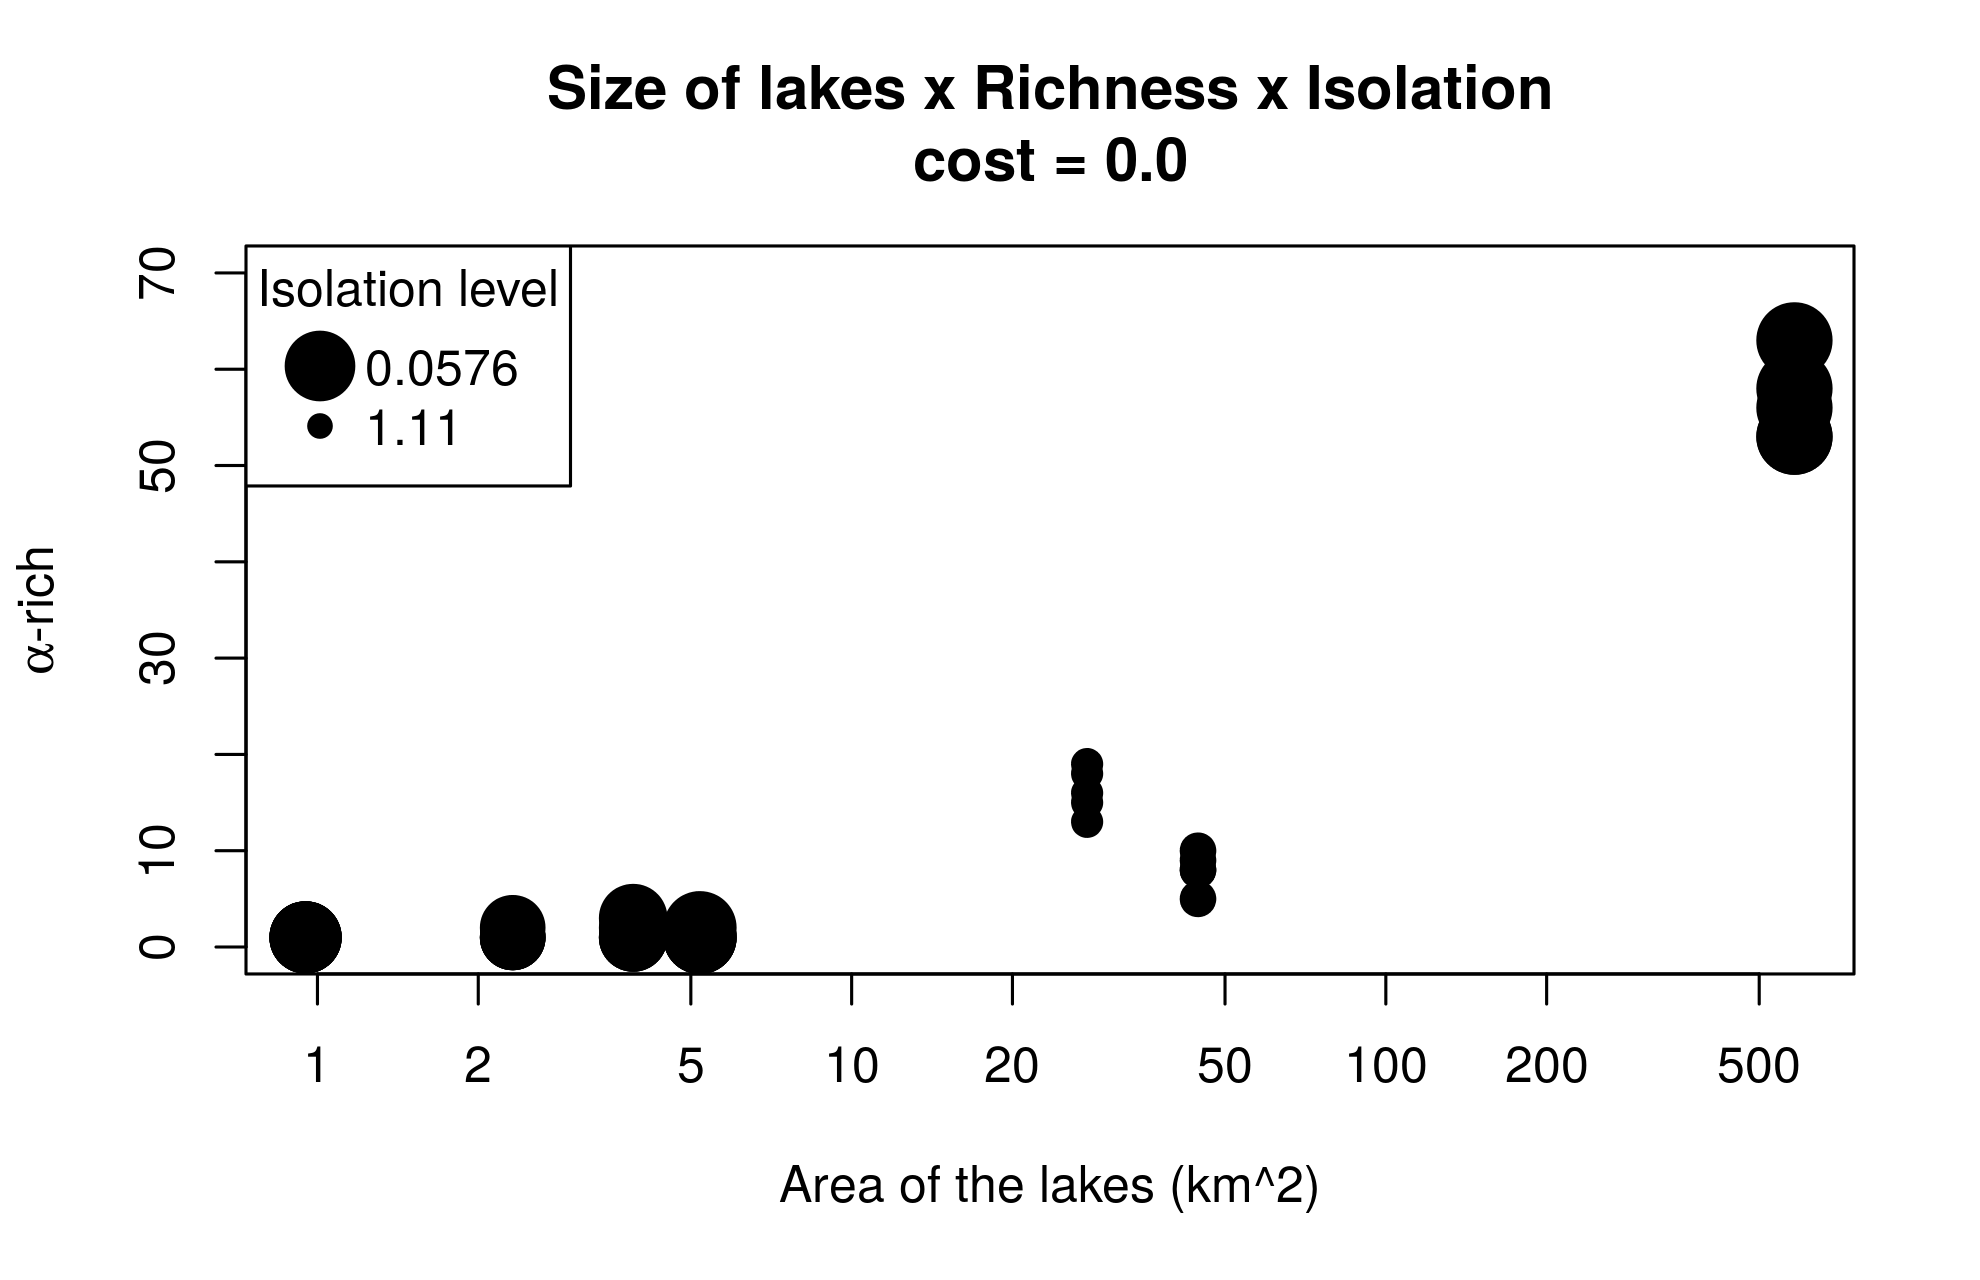
\includegraphics[width=0.9\linewidth]{images/RichnessSizeIsolationRichnessPerSiteAnaG20000cost0MR3e5VR6e6.png}}\\
\noindent{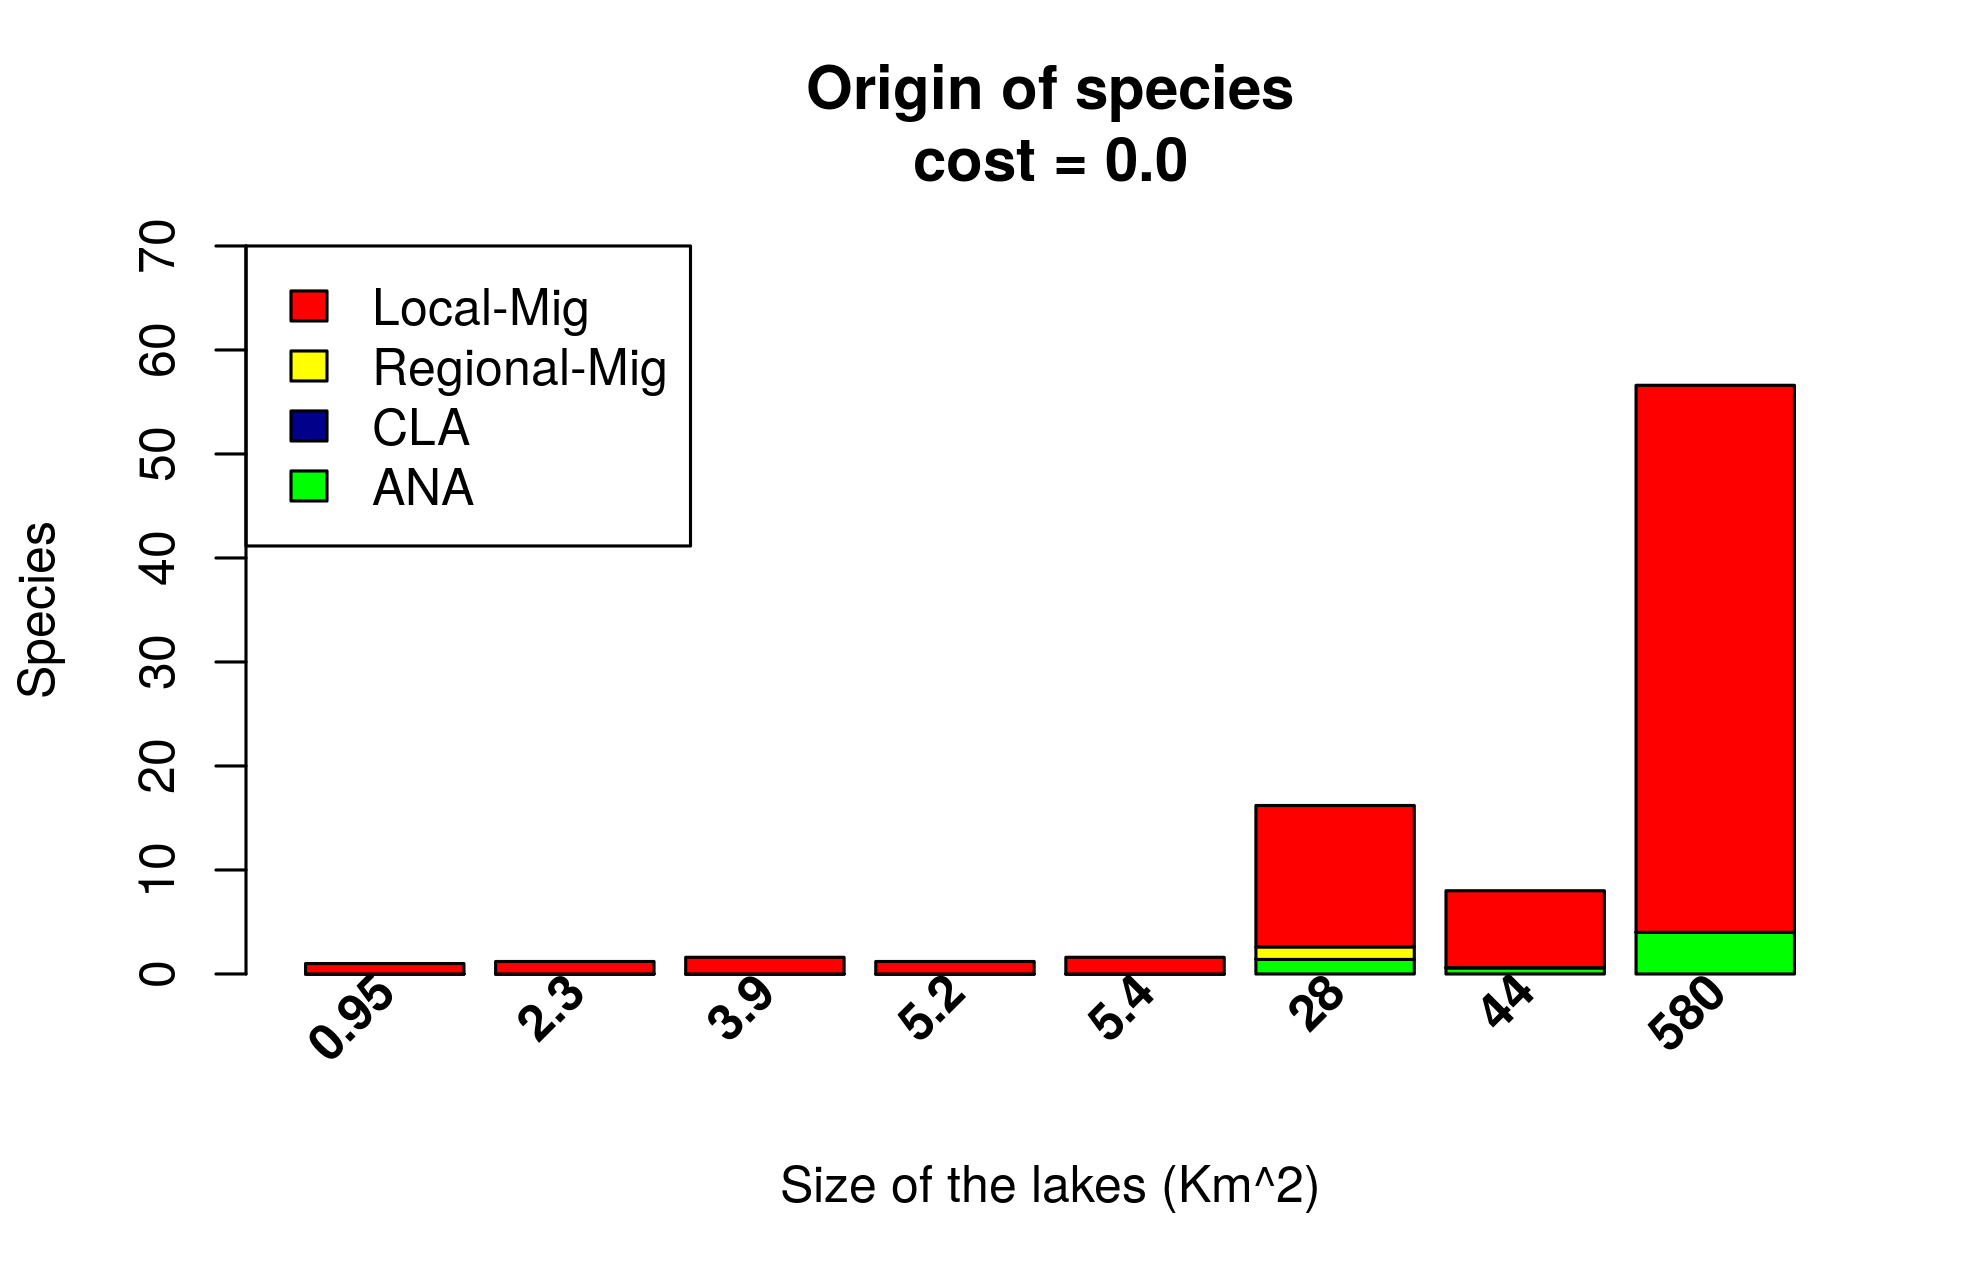
\includegraphics[width=0.9\linewidth]{images/SpeciationLakesRichnessPerSiteAnaG20000cost0MR3e5V6e6.png}}\\
{\bf C)} \noindent{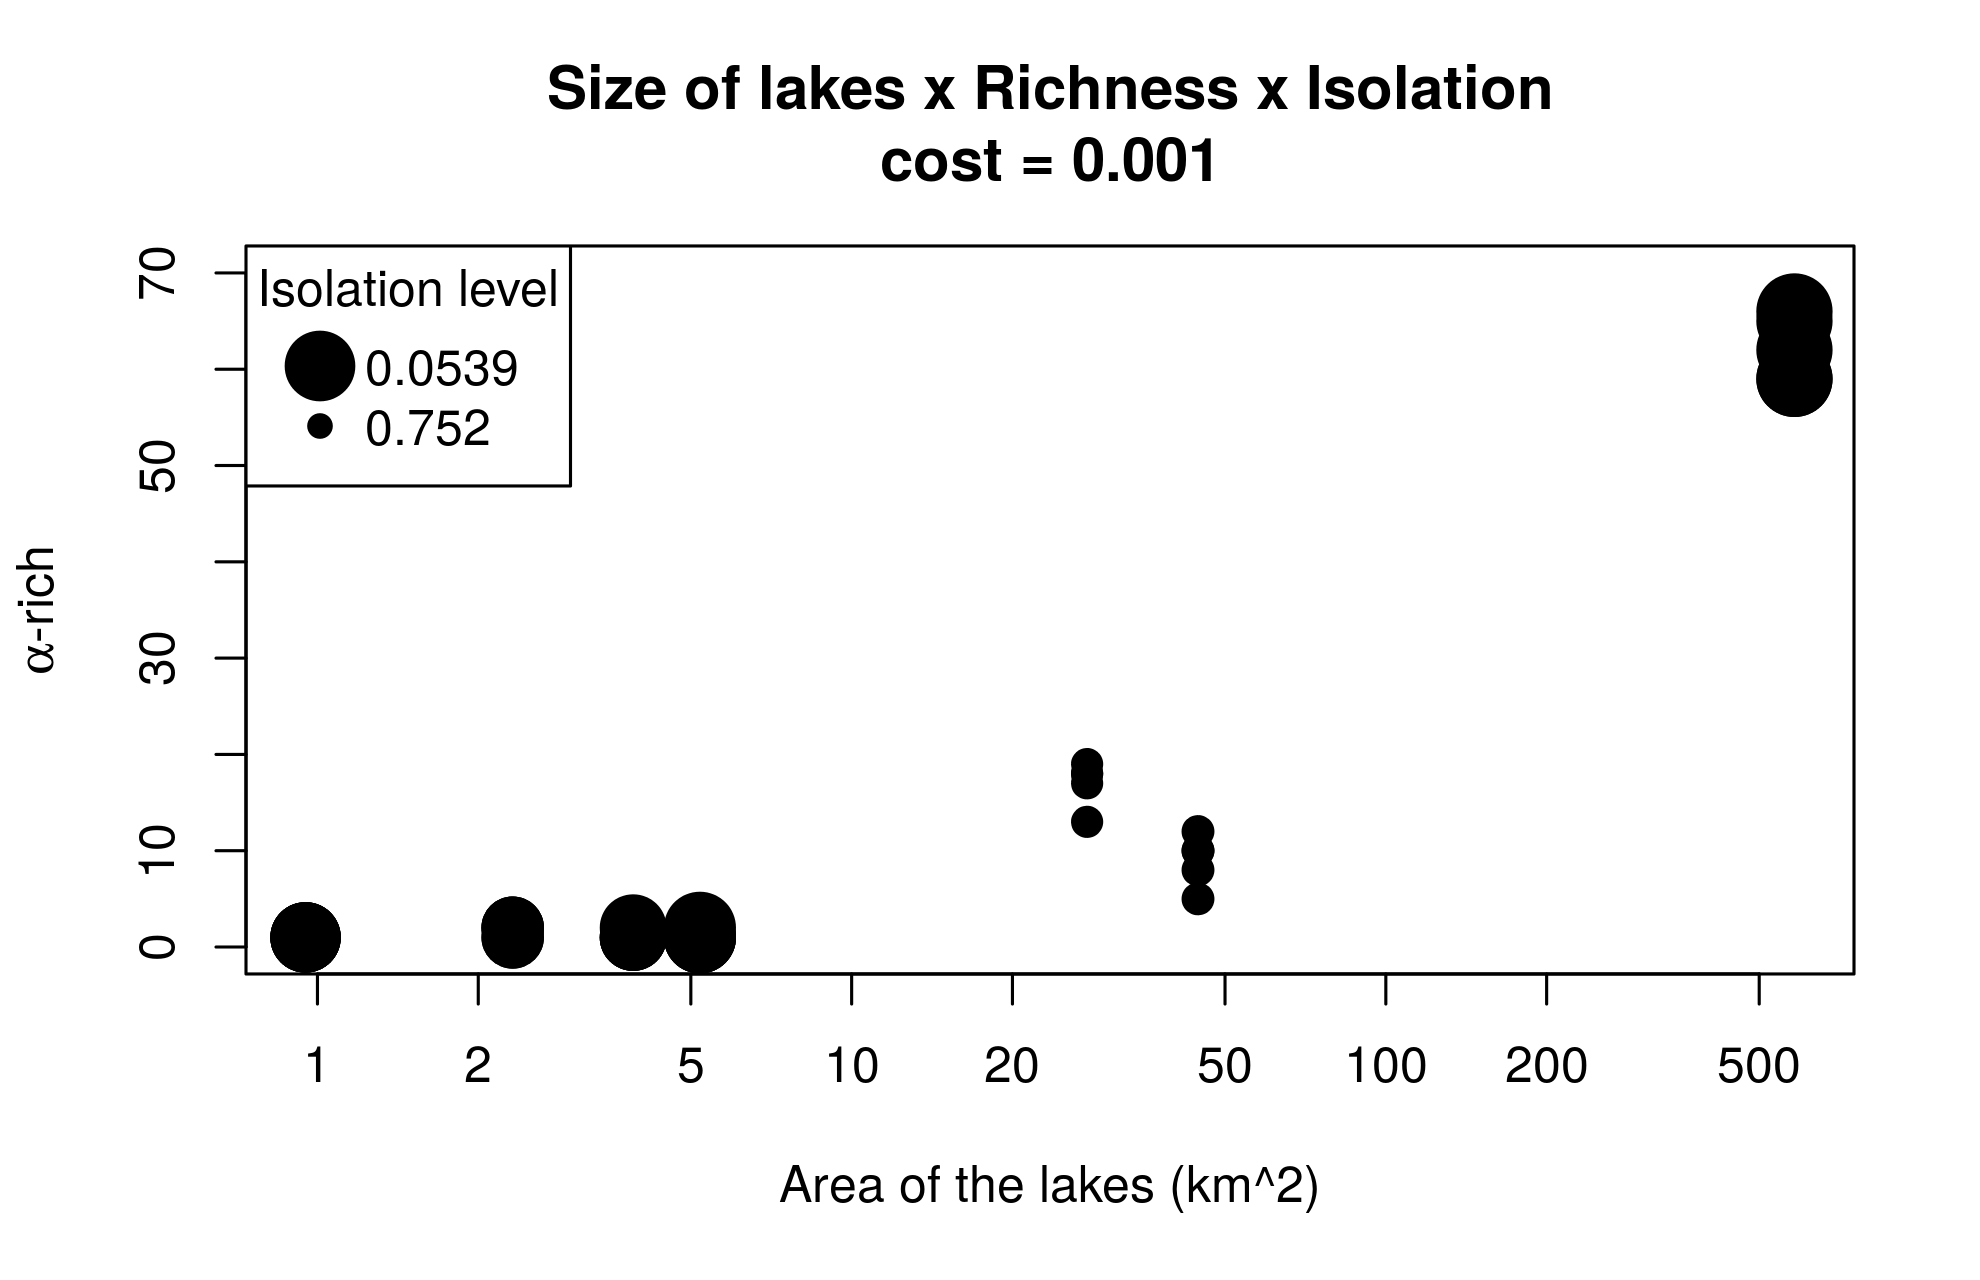
\includegraphics[width=0.9\linewidth]{images/RichnessSizeIsolationRichnessPerSiteAnaG20000cost0001MR6e5VR2e6.png}}\\
\noindent{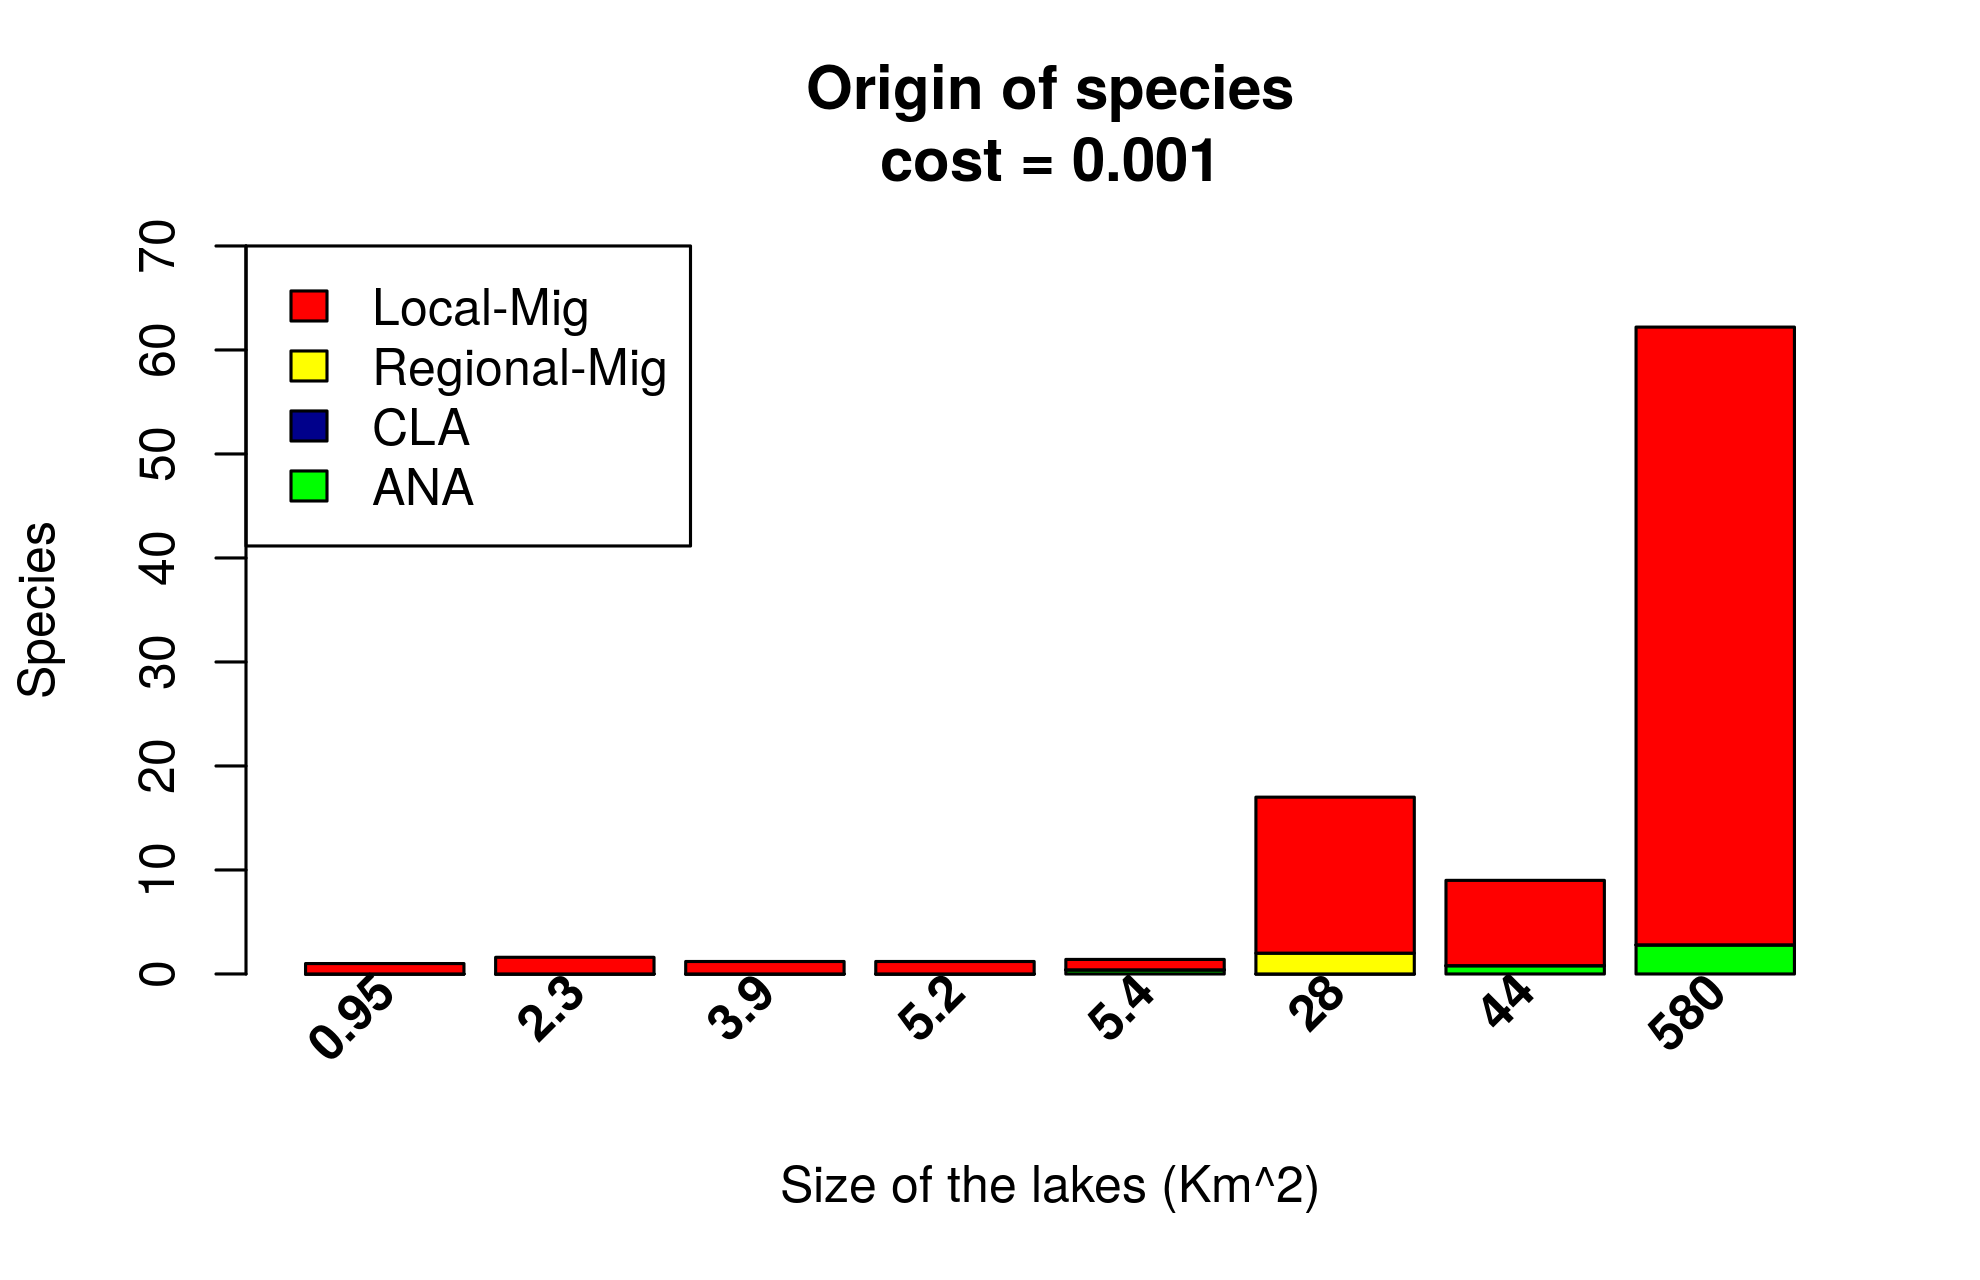
\includegraphics[width=0.9\linewidth]{images/SpeciationLakesRichnessPerSiteAnaG20000cost0001MR693e5VR2e6.png}}\\
 \end{multicols}
\vspace{-0.3 in} 
\caption{{\small {\bf A, top B and top C)} x- and y-axis represent the
    lake surface area and species richness, respectively. The
    species-area curve of the Rhone has a slope around 0.15, like the
    patterns in the observed dispersal-assemblies
    metacommunities. {\bf Top and bottom B and C} Represent
    predictions from our model. {\bf Top B and C} 10 replicates of the
    species-area curves show a nonlinear increase with lake size
    regardless upstream migration cost ({\bf Top B)} c=0, and {\bf Top
      C)} c=0.001). {\bf Bottom B and C} Show the proportion of
    species arriving to each lake from the local dendritic network
    (red), from regional migration (yellow, considering the lowest
    entry point in the network), cladogenesis (blue), and anagenesis
    (green). Upstream migration cost larger than zero decreases the
    number of anagenesis events but not the shape of the species-area
    curve (compare the largest lake between {\bf Bottom B and
      C}). Parameters used are: Number of individuals, $J$ =
    $10 X 10^{3}$, Number of generations per replicate, $10 X 10^{3}$,
    regional migration rate, $m_{r}$ = $1 X 10^{-5}$, local
    migration rate, $m_{l}$ = $2 X 10^{-3}$, cladogenesis speciation,
    $\nu_{c}$ = $1 X 10^{-6}$, anagenesis speciation, $\nu_{a}$ = $2$
    generations to speciation, the retardation parameter, $G$ = $1$
    generation, and the upstream migration cost, $c$ = $[0,0.001]$.}}
}
%%%%%%%%%%%%%%%%%%%%%%%%%%%%%%%%%%%%%%%%%%%%%%%%%%%%%%%%%%%%%%%%%%%%%%%%%%%%%%
%  \headerbox{References}{name=references,column=0,above=bottom}{
%%%%%%%%%%%%%%%%%%%%%%%%%%%%%%%%%%%%%%%%%%%%%%%%%%%%%%%%%%%%%%%%%%%%%%%%%%%%%%
%    \smaller
%    \bibliographystyle{ieee}
%    \renewcommand{\section}[2]{\vskip 0.05em}
%      \begin{thebibliography}{1}\itemsep=-0.01em
%      \setlength{\baselineskip}{0.4em}
%      \bibitem{amberg11:graphtrack}
%        B.~Amberg, T. Vetter.
%        \newblock {GraphTrack}: {F}ast and {G}lobally {O}ptimal {T}racking in {V}ideos
%        \newblock In {\em CVPR '11}
%      \bibitem{awf:tracking}
%        A.~Buchanan and A.~Fitzgibbon.
%        \newblock {I}nteractive {F}eature {T}racking using {K-D} {T}rees and {D}ynamic {P}rogramming.
%        \newblock In {\em CVPR '06}
%      \end{thebibliography}
%   \vspace{0.3em}
%  }
%%%%%%%%%%%%%%%%%%%%%%%%%%%%%%%%%%%%%%%%%%%%%%%%%%%%%%%%%%%%%%%%%%%%%%%%%%%%%%
  \headerbox{Future Direction}{name=questions,column=0,span=2,above=bottom}%,aligned=references,above=bottom}{
{
%%%%%%%%%%%%%%%%%%%%%%%%%%%%%%%%%%%%%%%%%%%%%%%%%%%%%%%%%%%%%%%%%%%%%%%%%%%%%%
  %\begin{multicols}{1}
  \vspace{2em} {\bf FUTURE DIRECTION} Model-data comparison with the
  Rhone drainage is so far qualitative. Our next step will be to use
  approximate Bayesian computation methods (ABC) to disentangle
  dispersal assembled communities with upstream migration cost from
  speciation assembled communities with clado and anagenesis
  speciation. ABC will allow us to fully explore the parameter space
  of the speciation modes and upstream migration cost using the
  $ProjetLac$ data for the Rhone, Rhine and Po drainages.
%\noindent{\centering \includegraphics[width=1\linewidth]{images/abc.pdf}\\}
  %\end{multicols}
   \vspace{0.3em}
  }
%%%%%%%%%%%%%%%%%%%%%%%%%%%%%%%%%%%%%%%%%%%%%%%%%%%%%%%%%%%%%%%%%%%%%%%%%%%%%%
  %\headerbox{Source Code}{name=references,column=3,aligned=references,above=bottom}{
%%%%%%%%%%%%%%%%%%%%%%%%%%%%%%%%%%%%%%%%%%%%%%%%%%%%%%%%%%%%%%%%%%%%%%%%%%%%%%
  %The source code...}

%%%%%%%%%%%%%%%%%%%%%%%%%%%%%%%%%%%%%%%%%%%%%%%%%%%%%%%%%%%%%%%%%%%%%%%%%%%%%%
  \headerbox{SAMPLING METHOD}{name=method,column=0,below=problem,}%bottomaligned=speed}{
{
%%%%%%%%%%%%%%%%%%%%%%%%%%%%%%%%%%%%%%%%%%%%%%%%%%%%%%%%%%%%%%%%%%%%%%%%%%%%%%
  \noindent{\centering \includegraphics[width=0.5\linewidth]{images/sampling.jpg}\\}
  \indent $ProjetLac$: Lakeshore and sublittoral habitats were mapped using
  boat-based observations. These maps formed the basis of the fish
  sampling, which involved a combination of habitat targeted ({\bf
    vertical gillnet protocol}) $\&$ stratified random ({\bf CEN})
  gillnets deployed in littoral, benthic and pelagic habitats. {\bf
    Electric fishing} was additionally used to capture slender and
  less mobile fish species in littoral shallow-water habitats.
  \vspace{0.3em} }

\end{poster}
\end{document}
